\documentclass[12pt]{article}

\usepackage{graphicx}
\usepackage[margin=0.75in]{geometry}
\usepackage{multirow}

\usepackage{amsmath}
\usepackage{bm}
\newcommand{\m}[1]{\mathbf{\bm{#1}}}

\begin{document}

\section*{AMS 276 -- Project 1}
\subsection*{Mickey Warner}
\bigskip
\bigskip

\section*{Frailty model}

\noindent For observation $i$ and measurement $j$, we assume the hazard at time $y_{ij}$ is given by
\[ h(y_{ij}|\m{x}_{ij}, w_i) = h_0(y_{ij})w_i\exp(\m{x}_{ij}^\top\m{\beta}),~~~i=1,\ldots,n,~~~j=1,\ldots,m_i \] 
\noindent The covariates $\m{x}_{ij}$ is a vector of length 2. The first element is the sex (1 for female, 0 for male) and the second is age. We assume the baseline hazard $h_0$ is a Weibull, i.e. $h_0(t)=\alpha\gamma t^{\alpha-1}$. This yields the following likelihood
\begin{eqnarray*}
L(\m{y}|\m{x},\m{\nu},\m{w},\alpha,\gamma,\m{\beta}) &=& \prod_{i=1}^n \prod_{j=1}^{m_i} \left[h(y_{ij}|\m{x}_{ij},w_i)\right]^{\nu_{ij}} \exp\left(-H(y_{ij}|\m{x}_{ij},w_i)\right) \\
 &=& \prod_{i=1}^n \prod_{j=1}^{m_i} \left[h_0(y_{ij})w_i\exp(\m{x}_{ij}^\top\m{\beta})\right]^{\nu_{ij}} \exp\left(-H_0(y_{ij})w_ie^{\m{x}_{ij}^\top\m{\beta}}\right) \\
 &=& \prod_{i=1}^n \prod_{j=1}^{m_i} \left[\alpha\gamma y_{ij}^{\alpha-1}w_i\exp(\m{x}_{ij}^\top\m{\beta})\right]^{\nu_{ij}} \exp\left(-\gamma y_{ij}^\alpha w_ie^{\m{x}_{ij}^\top\m{\beta}}\right)
\end{eqnarray*}

\subsection*{Priors}

\noindent We assume the following priors
\begin{eqnarray*}
w_i | \kappa &\overset{iid}\sim& Gamma(\kappa^{-1},\kappa^{-1}) \\
\eta = \kappa^{-1} &\sim& Gamma(\phi_1,\phi_2) \\
\m{\beta} &\sim& Normal(\bar{\m{\beta}}, \m{\Sigma}) \\
\gamma &\sim& Gamma(\rho_1,\rho_2) \\
\alpha &\sim& Gamma(a_1, a_2)
\end{eqnarray*}
\noindent Equivalent, we could let $\kappa \sim InvGamma(\phi_1,\phi_2)$. We take this approach since there were some issues in sampling $\eta$ because of a very long right tail. We let $\phi_1=\phi_2=0.001$, $\bar{\m{\beta}}=\m{0}$, $\m{\Sigma}=10^3 \m{I}_{2\times 2}$, $\rho_1=\rho_2=0.001$, and $a_1=a_2=0.001$.

\subsection*{Full conditionals}

\noindent The full posterior is
\begin{eqnarray*}
\pi(\m{w},\gamma,\kappa,\m{\beta},\alpha|\cdot) \propto \left\{\prod_{i=1}^n \prod_{j=1}^{m_i} \left[\alpha\gamma y_{ij}^{\alpha-1}w_i\exp(\m{x}_{ij}^\top\m{\beta})\right]^{\nu_{ij}} \exp\left(-\gamma y_{ij}^\alpha w_ie^{\m{x}_{ij}^\top\m{\beta}}\right)\right\} \times \\
\left\{\prod_{i=1}^n \frac{(\kappa^{-1})^{\kappa^{-1}}}{\Gamma(\kappa^{-1})}w_i^{\kappa^{-1}-1}\exp(-w_i\kappa^{-1})\right\} \times \kappa^{-(\phi_1+1)}\exp\left(-\frac{\phi_2}{\kappa}\right) \times \\
\exp\left(-\frac{1}{2}(\m{\beta}-\bar{\m{\beta}})^\top\m{\Sigma}^{-1}(\m{\beta}-\bar{\m{\beta}})\right) \times \gamma^{\rho_1-1}\exp\left(-\gamma\rho_2\right) \times \\
\alpha^{a_1-1}\exp\left(-\alpha a_2\right)
\end{eqnarray*}

\noindent We now derive the full conditionals for each parameter.

\begin{eqnarray*}
\pi(w_i|\cdot) &\propto& \prod_{j=1}^{m_i} w_i^{\nu_{ij}}\exp\left(-\gamma y_{ij}^\alpha w_ie^{\m{x}_{ij}^\top\m{\beta}}\right) \times w_i^{\kappa^{-1}-1}\exp(-w_i\kappa^{-1}) \\
&=& w_i^{\sum_{j=1}^{m_i}\nu_{ij}}\exp\left(-w_i \sum_{j=1}^{m_i}\gamma y_{ij}^\alpha e^{\m{x}_{ij}^\top\m{\beta}}\right) \times w_i^{\kappa^{-1}-1}\exp(-w_i\kappa^{-1}) \\
&=& w_i^{(\kappa^{-1}+\sum_{j=1}^{m_i}\nu_{ij})-1}\exp\left(-w_i(\kappa^{-1}+\sum_{j=1}^{m_i}\gamma y_{ij}^\alpha e^{\m{x}_{ij}^\top\m{\beta}})\right) \\
&\implies& w_i|\cdot \sim Gamma\left(\kappa^{-1}+\sum_{j=1}^{m_i}, \kappa^{-1}+\sum_{j=1}^{m_i}\gamma y_{ij}^\alpha e^{\m{x}_{ij}^\top\m{\beta}}\right) \\
\\ \\
\pi(\gamma|\cdot) &\propto& \left\{\prod_{i=1}^n \prod_{j=1}^{m_i} \gamma ^{\nu_{ij}} \exp\left(-\gamma y_{ij}^\alpha w_ie^{\m{x}_{ij}^\top\m{\beta}}\right)\right\} \times \gamma^{\rho_1-1}\exp(-\gamma\rho_2) \\
 &=& \gamma^{\sum_{i=1}^n\sum_{j=1}^{m_i}\nu_{ij}} \exp\left(-\gamma \sum_{i=1}^n\sum_{j=1}^{m_i}y_{ij}^\alpha w_ie^{\m{x}_{ij}^\top\m{\beta}}\right) \times \gamma^{\rho_1-1}\exp(-\gamma\rho_2) \\
 &=& \gamma^{(\rho_1+\sum_{i=1}^n\sum_{j=1}^{m_i}\nu_{ij})-1} \exp\left(-\gamma(\rho_2+ \sum_{i=1}^n\sum_{j=1}^{m_i}y_{ij}^\alpha w_ie^{\m{x}_{ij}^\top\m{\beta}})\right) \\
 &\implies& \gamma|\cdot \sim Gamma\left(\rho_1+\sum_{i=1}^n\sum_{j=1}^{m_i}\nu_{ij}, \rho_2+ \sum_{i=1}^n\sum_{j=1}^{m_i}y_{ij}^\alpha w_ie^{\m{x}_{ij}^\top\m{\beta}}\right) \\
\\ \\
\pi(\kappa|\cdot) &\propto& \left\{\prod_{i=1}^n \frac{(\kappa^{-1})^{\kappa^{-1}}}{\Gamma(\kappa^{-1})}w_i^{\kappa^{-1}-1}\exp(-w_i\kappa^{-1})\right\} \times \kappa^{-(\phi_1+1)}\exp\left(-\frac{\phi_2}{\kappa}\right) \\
\\ \\
\pi(\m{\beta}|\cdot) &\propto& \left\{\prod_{i=1}^n \prod_{j=1}^{m_i} \left[\exp(\m{x}_{ij}^\top\m{\beta})\right]^{\nu_{ij}} \exp\left(-\gamma y_{ij}^\alpha w_ie^{\m{x}_{ij}^\top\m{\beta}}\right)\right\} \times \exp\left(-\frac{1}{2}(\m{\beta}-\bar{\m{\beta}})^\top\m{\Sigma}^{-1}(\m{\beta}-\bar{\m{\beta}})\right) \\
\\ \\
\pi(\alpha|\cdot) &\propto& \left\{\prod_{i=1}^n \prod_{j=1}^{m_i} \left[\alpha y_{ij}^{\alpha-1}\right]^{\nu_{ij}} \exp\left(-\gamma y_{ij}^\alpha w_ie^{\m{x}_{ij}^\top\m{\beta}}\right)\right\} \times \alpha^{a_1-1}\exp(-\alpha a_2)
\end{eqnarray*}
\bigskip

\noindent We will use Metropolis-Hastings updates for $\m{\beta}$, $\kappa$, and $\alpha$, while we can sample directly for each $w_i$ and $\gamma$. After a significant burn-in, we retain $200,000$ posterior samples. Trace plots on the posteriors of $\m{\beta}$, $\kappa$, and $\alpha$ showed no concern of convergence. Acceptance rates for the M-H parameters were around $0.20-0.26$, a desirable range. Chains that started at various starting locations all ended up in the same location.

\section*{Results and interpretation of parameters}

\noindent Posterior distributions are given in Figures 1 and 2. A summary for $\kappa$, $\m{\beta}$, $\gamma$, and $\alpha$ are shown in Table 1. My posteriors are very comparable to those given in your analysis.
\bigskip

\begin{table}[ht]
\centering
\begin{tabular}{lcrrrr}
\hline\hline
& & \multicolumn{1}{l}{mean} & \multicolumn{1}{l}{sd} &
    \multicolumn{1}{l}{$0.025\%$} & \multicolumn{1}{l}{$0.975\%$} \\ \hline
$\kappa $ & & $ 0.600$ & $0.307$ & $ 0.125$ & $ 1.324$ \\
$\beta_1$ & & $-1.937$ & $0.576$ & $-3.147$ & $-0.865$ \\
$\beta_2$ & & $ 0.007$ & $0.013$ & $-0.017$ & $ 0.034$ \\
$\gamma $ & & $ 0.017$ & $0.015$ & $ 0.002$ & $ 0.057$ \\
$\alpha $ & & $ 1.234$ & $0.162$ & $ 0.931$ & $ 1.578$ \\
\hline\hline
\end{tabular}
\caption{Posterior summaries for some parameters.}
\end{table}

\noindent $\kappa$ describes the homogeneity of the cluster frailties. For a new cluster $w^\star$, the predictive mean is $1$, and the predictive variance is $\kappa^\star$, where $\kappa^\star$ is the posterior for $\kappa$. So for small $\kappa$, the clusters are more similar. For large $\kappa$, we would see more $w_i$'s that are much different than the rest, but this is not quite the case from our analysis.
\bigskip

\noindent The parameters $(\gamma,\alpha)$ are from the Weibull distribution. Here, they may best be interpreted relative to their role in the hazard function. There is good evidence that $\alpha>1$, meaning as time goes on, the hazard increases. $\gamma$ is a scale parameter so no one cares about it.
\bigskip

\noindent The parameters $(\beta_1,\beta_2)$ can be used to compare survival times for the male and female groups as well as for the age of the subjects. Using the posterior samples of $\beta_1$, we compute $E(e^{\beta_1})=0.168$. This means that the hazard function for females is $0.168$ times that as for the males. There is weak evidence that $\beta_2>0$, which is to say that as age increases, the hazard function increases.

\bigskip

\noindent We also fit a frequentist model in R:
\smallskip

\noindent \texttt{coxph(Surv(time, nu) $\sim$ as.factor(Sex) + Age + frailty(cluster, theta = 1), \\
data = data.frame(dat))}
\smallskip

\noindent We fix $\kappa=\theta=1$, which is comparable to our prior that $w_i$ has prior mean 1.

\begin{table}[ht]
\centering
\begin{tabular}{lcrr}
\hline\hline
& & \multicolumn{1}{l}{m.l.e.} & \multicolumn{1}{l}{s.e.} \\
$\beta_1$: Female   & & $-1.93574$ & $0.58022$ \\
$\beta_2$: Age      & & $ 0.00832$ & $0.01577$ \\
\hline\hline
\end{tabular}
\caption{Frequentist estimates for $\beta_1$ and $\beta_2$.}
\end{table}


\noindent These estimates are very similar to ours. But it isn't Bayesian so it's obviously not as good. Plus, the algorithm broke when I didn't fix $\kappa$.


\newpage
\begin{figure}
\centering
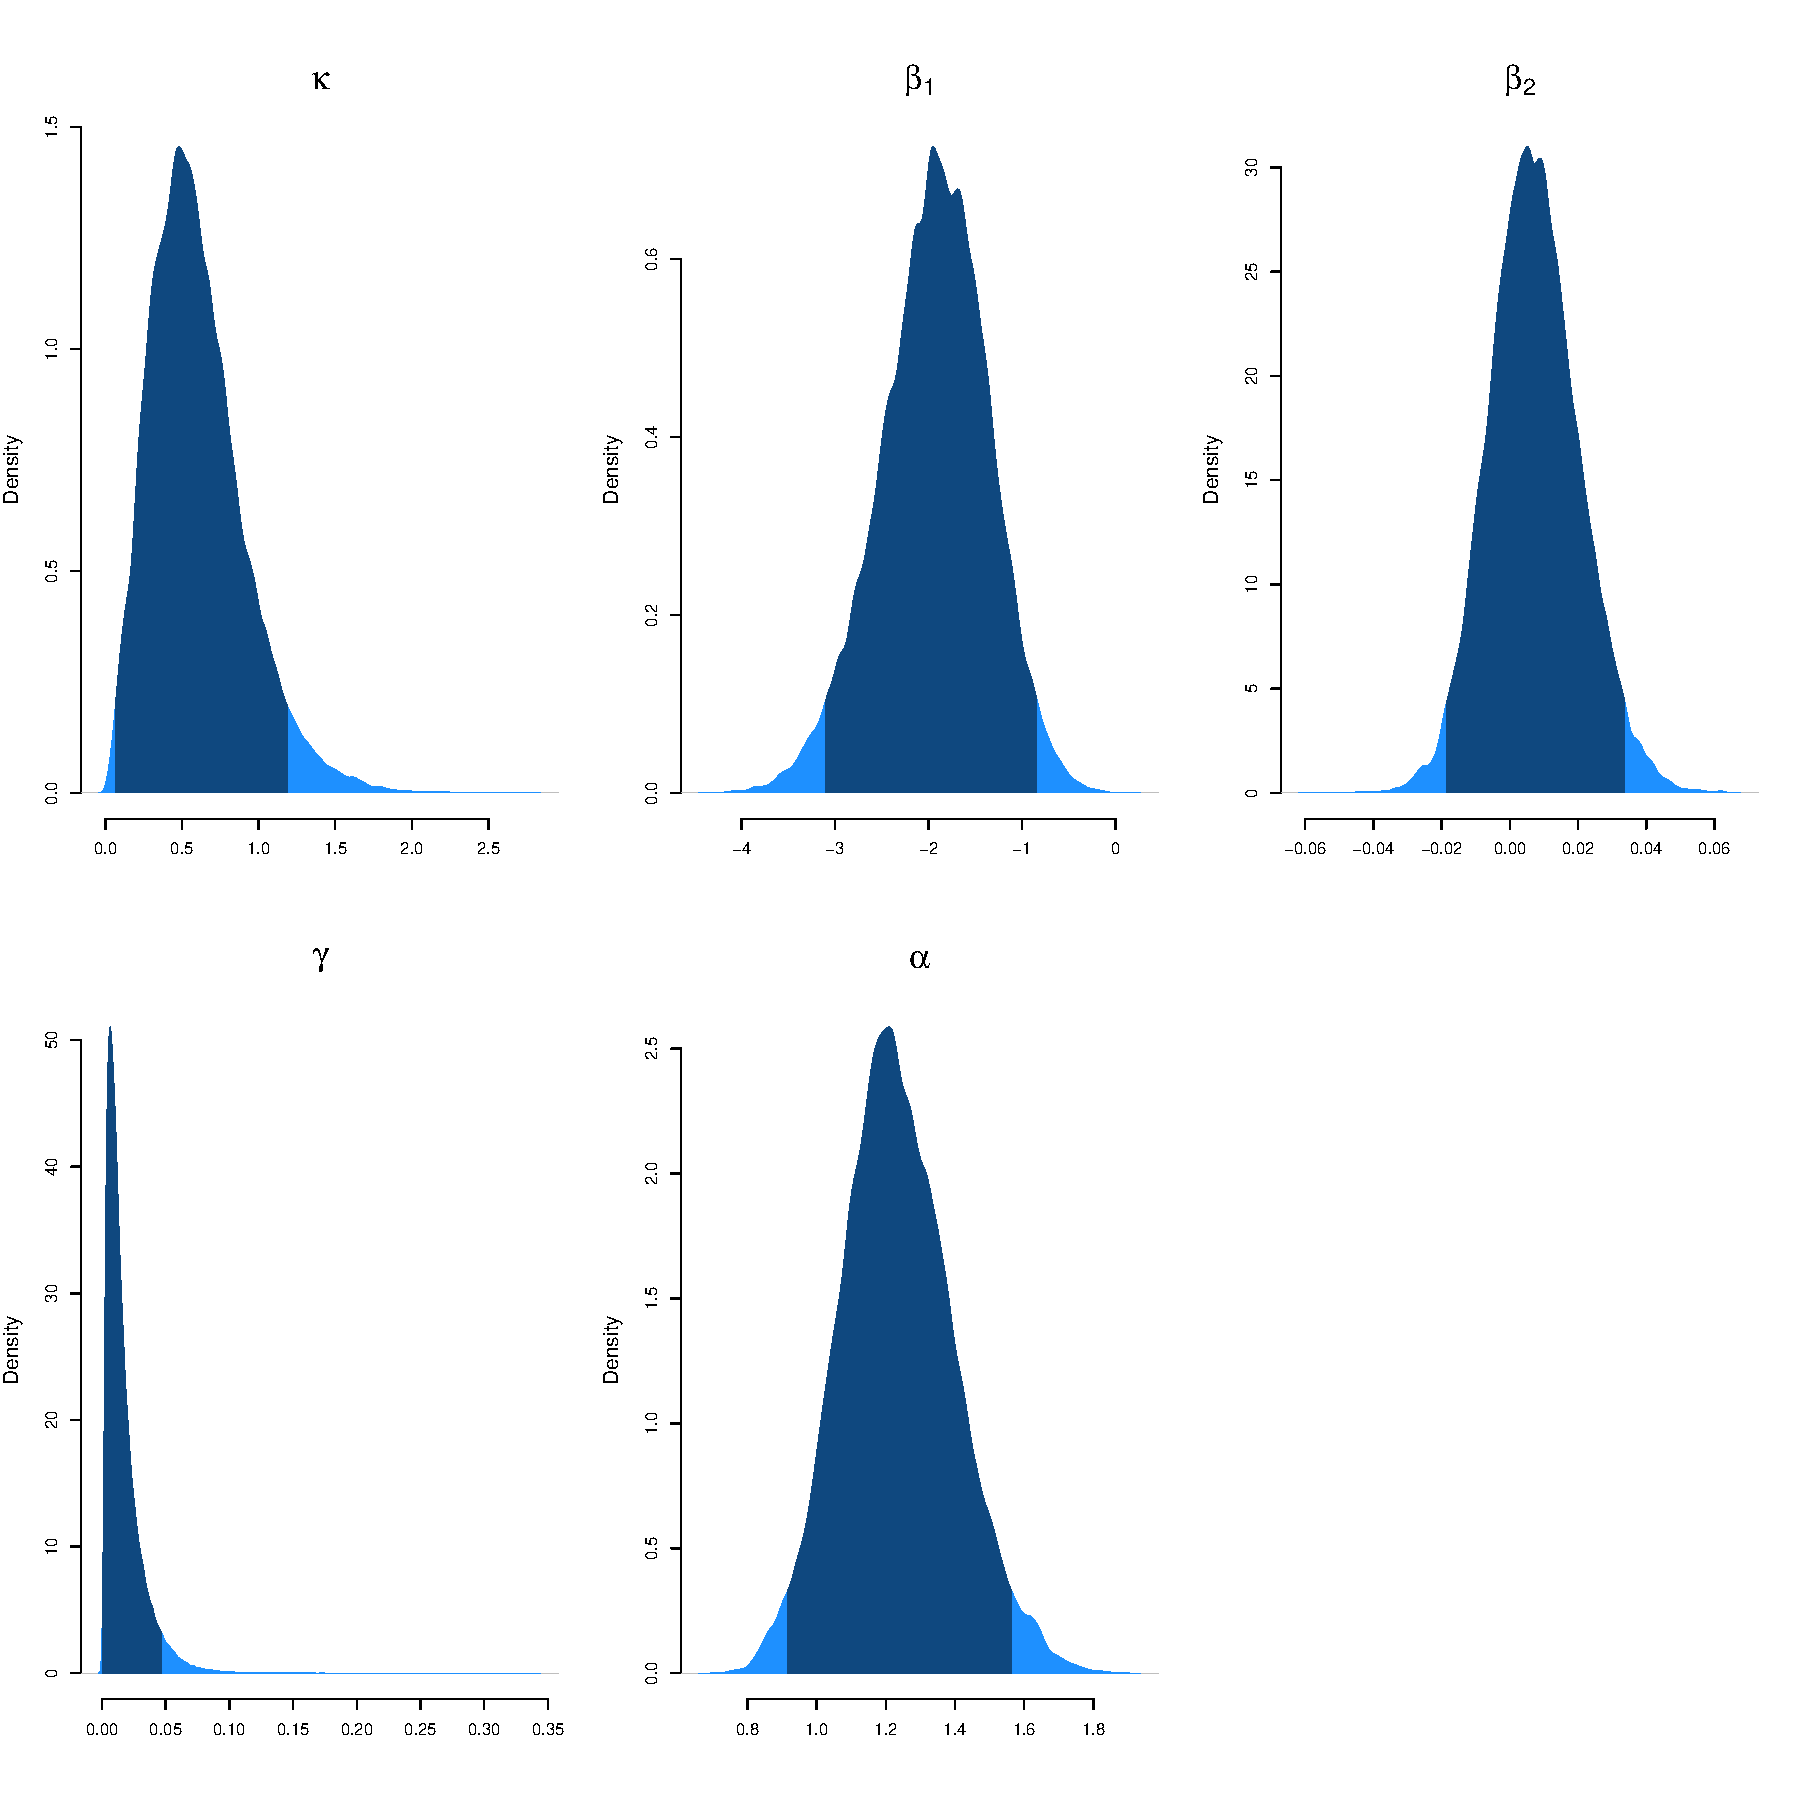
\includegraphics[scale=0.5]{figs/posterior.pdf}
\caption{Posterior distributions and summary statistics for $\kappa$, $\m{\beta}$, $\gamma$, and $\alpha$.}
\end{figure}

\begin{figure}
\centering
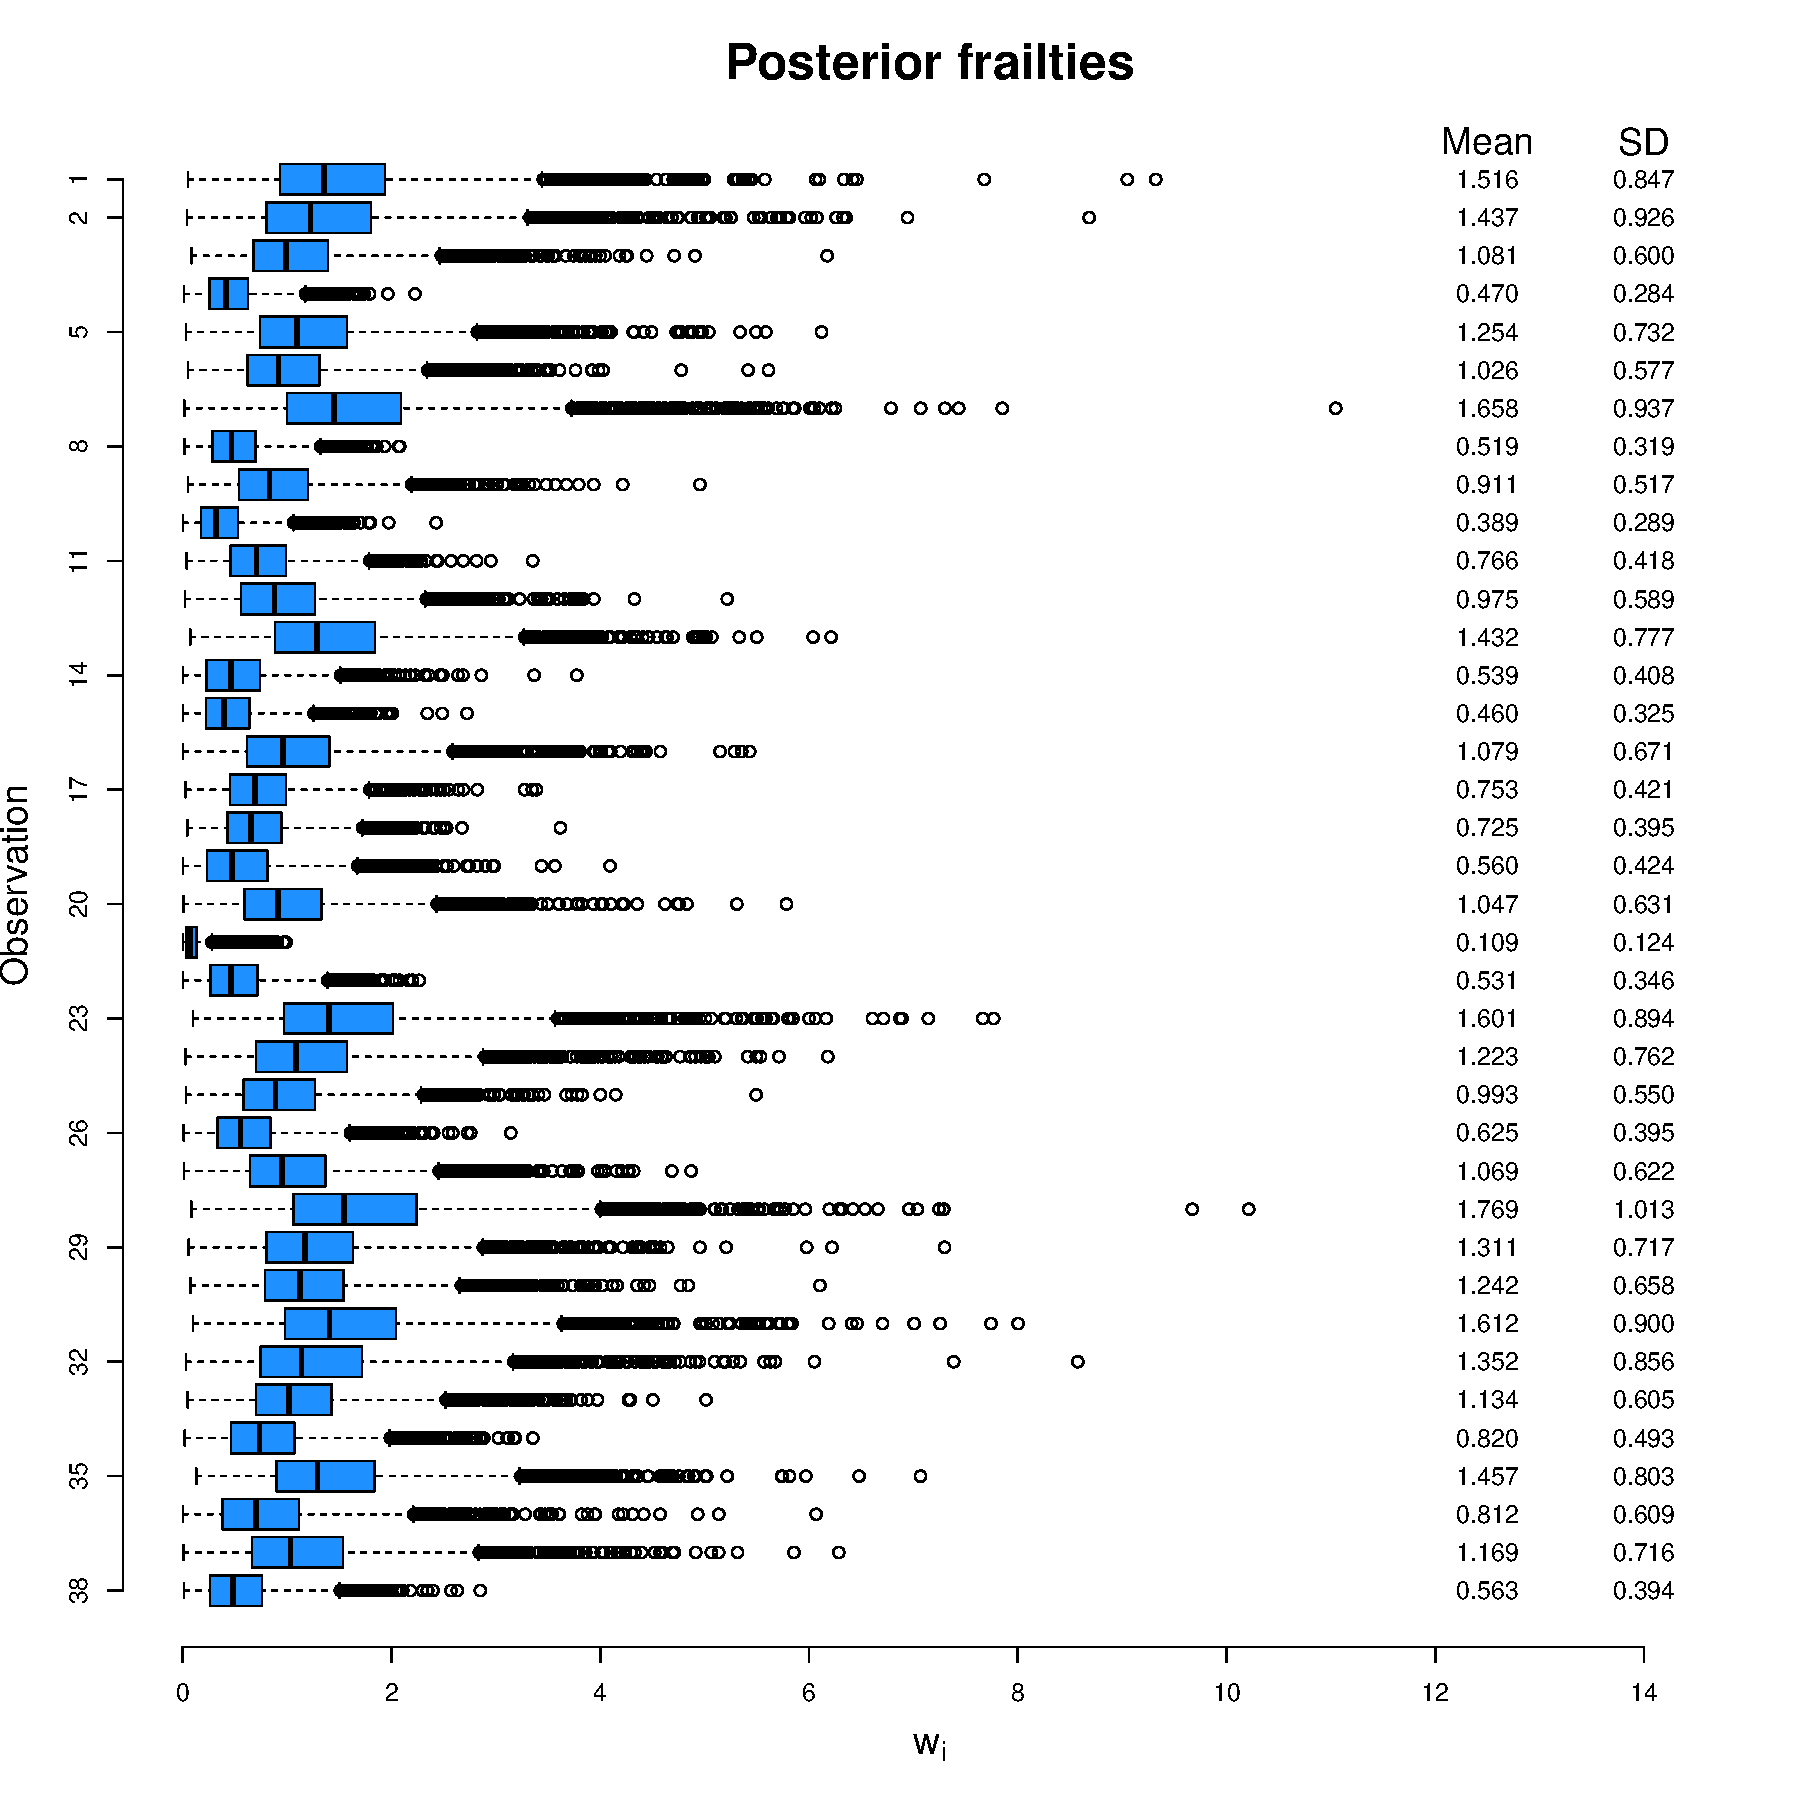
\includegraphics[scale=0.5]{figs/frailty.pdf}
\caption{Boxplots for the $n=38$ frailty parameters $w_i$ with mean and standard deviations.}
\end{figure}

\end{document}
